\documentclass{article}
\usepackage{graphicx}

\begin{document}

% Slide 1
\title{Deploying predictive models with the Actor framework}
\author{Brian Gawalt}

\maketitle

% Slides 2 - 6

\begin{abstract}
The majority of data science and machine learning tutorials focus on generating models: assembling a dataset; splitting the data into training, validation, and testing subsets; building the model; and demonstrating its generalizability. But when it's time to repeat the analogous steps when using the model in production, issues of high latency or low throughput can arise. To an end user, the cost of too much time spent featurizing raw data and evaluating a model over features can wind up erasing any gains a smarter prediction can offer. 

Exposing concurrency in these model-usage steps, and then capitalizing on that concurrency, can improve throughput. This work describes how the Actor framework can be used to bring a predictive model to a real-time setting. Two case-study examples are described: a simple text classifier (with accompanying code), and a live deployment built for the freelancing platform Upwork.
\end{abstract}

\section{The practice of machine learning}

Imagine a firm has brought a specialist in machine learning onto a new project. The firm wants a product which can provide a quality prediction about some regular event happening in the course of the firm's business. The specialist is handed a pile of relevant historical data, and asked: Among the new customers seen for the first time today, who's likeliest to be a big spender? Or: of all the credit card transactions processed in the last hour, which are likeliest to be fraudulent? Or: when a customer enters a query into our website's Search tool, what results should we be returning?

The specialist starts with the first of two phases of the work. They have to identify a model that can be expected to fit predictions over both the historical data and in a way that will generalize to new data. The familiar version of the steps involved in supervised learning: 

\begin{enumerate}
\item Identify raw source data, and break it down into distinct observations of the pattern you're trying to learn and predict.
\item For each raw observation, produce a $p$-dimensional vector of features and a scalar label.
\item Split this collection into disjoint training, validation, and testing sets.
\item For each candidate model (and/or each hyperparameter value of the model/models), fit model parameters to the training vectors and labels, and evaluate the goodness of fit by performing prediction of the validation labels given the validation vectors
\item Select the model whose validation-set predictions came closest to the mark. Use it to then make predictions over the test set. Report this test set performance to vouch for the predictive model you've generated and selected.
\end{enumerate}

Note that this first phase doesn't carry an explicit component of \emph{time urgency}. All else equal, a typical specialist will prefer that the full sequence complete in six hours, and six minutes is better still. But if it takes six days instead, nothing \emph{fundamental} to this first phase has been threatened. The task -- finding a model that generates acceptably accurate predictions on new data -- is accomplished.

The second phase is to actually put the model's capabilities to use. Given new events and observation that need scoring by the model -- is this new customer likely to be a big spender? is this credit card legitimate? -- the above featurization and scoring routines need to be run. And in this real-world deployment, it's likely that there are also some strict constraints on how long it takes this sequence to run. All predictions go stale, and some use cases need to act on a prediction within milliseconds of the event itself.

There are some cases where these latency constraints aren't binding. The exact same featurization and scoring routines used to generate and validate the model can be re-run fast enough on new data to produce useful predictions. But this work focuses on the cases where timeliness requirements exclude the use of the same software developed in the first phase as the backbone of the second phase. What can a lone machine learning specialist do to retool their sequence to run in a production environment?

\subsection{Moving to production}

If the original software, used to generate and validate the predictive model, is suffering from too-low throughput in producing new predictions, one path forward could be to incorporate more concurrent processing. The three steps to prediction (gathering raw materials, featurizing those materials into vectors, scoring the vectors) can transition from a serial sequence to a pipeline.

 Figure 1 demonstrates a modification of the scoring task flow, producing predictions of $N$ events in a sequential and a concurrent pattern.  This pipeline offers a few advantages. Scores are produced with less delay after the raw material gathering (useful in case the information in that material is at risk of going stale or out of date). 
 
 \begin{figure}[h]
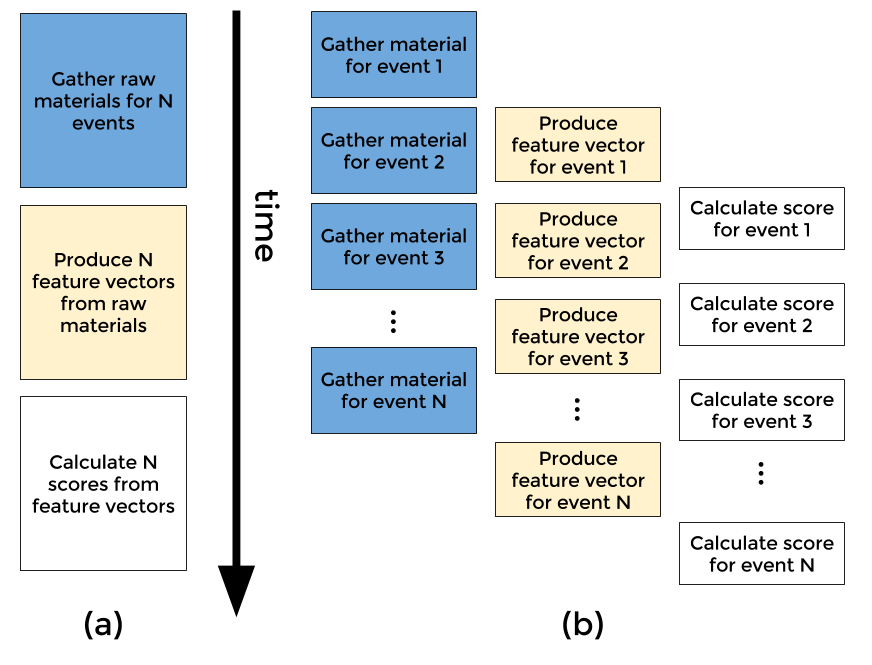
\includegraphics[width=0.6\textwidth]{fig/tex/pipeline.png}
\centering
\caption{(a) The scoring procedure performed serially. (b) The individual tasks for each event to be scored performed in a concurrent pipeline.}
\end{figure}

Most importantly, this redesign provides a clear path forward to speed-up in completing all $N$ scoring tasks. If a system can genuinely perform the concurrent tasks in parallel, as a multicore system might, one can easily picture adding ``clones'' of this pipeline simultaneously processing more and more partitions of the $N$ events.







\end{document}